% \subsection{問題設定}
% 本研究では,銀行のローンの審査システムについての機械学習モデルを想定し,認可拒否について誤分類を引き起こす敵対的サンプルを生成することを考える.銀行のローンを申請する顧客情報と正解データをもとに機械学習モデルが学習し,テストデータに対する分類結果を出力する.敵対的サンプルによる誤分類は,銀行にとってリスクの高いローンを誤って認可してしまう可能性がある.このような問題に対処するため,機械学習モデルの安全性が求められており,敵対的サンプルに対する防御手法が必要である.また同時に,モデルの脆弱性を理解することは,安全性を向上させるために重要である.

\subsection{敵対的学習}
\subsubsection{敵対的学習の概要}
機械学習モデルは,膨大なデータからパターンを学習し,予測や分類を行う.しかし,そのデータに微小な変更(敵対的サンプル)が加えられることで,人間には明らかに正しいと認識されるデータを,モデルが誤分類してしまうケースがある.これにより,安全性が求められる分野(例:顔認証や金融審査など)で深刻な問題が発生する可能性があります.

敵対的学習は,機械学習モデルの堅牢性を向上させるための手法として誕生した.従来の機械学習モデルは,訓練データに対して高い精度を示す一方で,敵対的サンプルと呼ばれる微細ななノイズを含むデータに対しては脆弱である.

goodfellowらの研究\cite{goodfellow2015explaining}でこの敵対的学習について提案された.この手法では,正常データと敵対的サンプルの特徴をAIに学習させる防御手法である.機械学習モデルの学習時において,正常データと敵対的サンプルに対する誤差(Loss)をそれぞれ計算する。以下の式(1)のように先ほどの誤差を足し合わせ、これらを基にモデルの重み $\bm{w}$ を更新し,敵対的サンプルの特徴を学習する.

\autoequation{\alpha \cdot Loss(x,y) + (1-\alpha) \cdot Loss(\tilde{x},y)}

ここで、$\alpha$ は元データと敵対的サンプルの誤差のバランスを調整するパラメータであり、$Loss(x,y)$ は元データ $x$ とラベル $y$ に対する誤差、$Loss(\tilde{x},y)$ は敵対的サンプル $\tilde{x}$ とラベル $y$ に対する誤差を表します。

\subsubsection{敵対的学習の流れ}
以下に実際の敵対的学習の流れを示す.\cite{MBSD-AdversarialTraining}

\begin{enumerate}

    \item 学習中の機械学習モデルを利用して敵対的サンプルを作成する

    下に示す図1は,敵対的学習の最初のステップである,元データから敵対的サンプルを作成するプロセスを示している.この図では,元画像に微細なノイズを加えることで,モデルが誤分類を引き起こす敵対的サンプルが生成される様子を視覚的に表している.最初に元データの画像を機械学習モデルに入力し,予測ラベル $y$ を得る.次に,この予測と正解データを比較した誤差を $Loss$ 関数で計算し,この誤差を最小化するように敵対的サンプルを生成している.
    
    \begin{figure}[H]
        \centering
        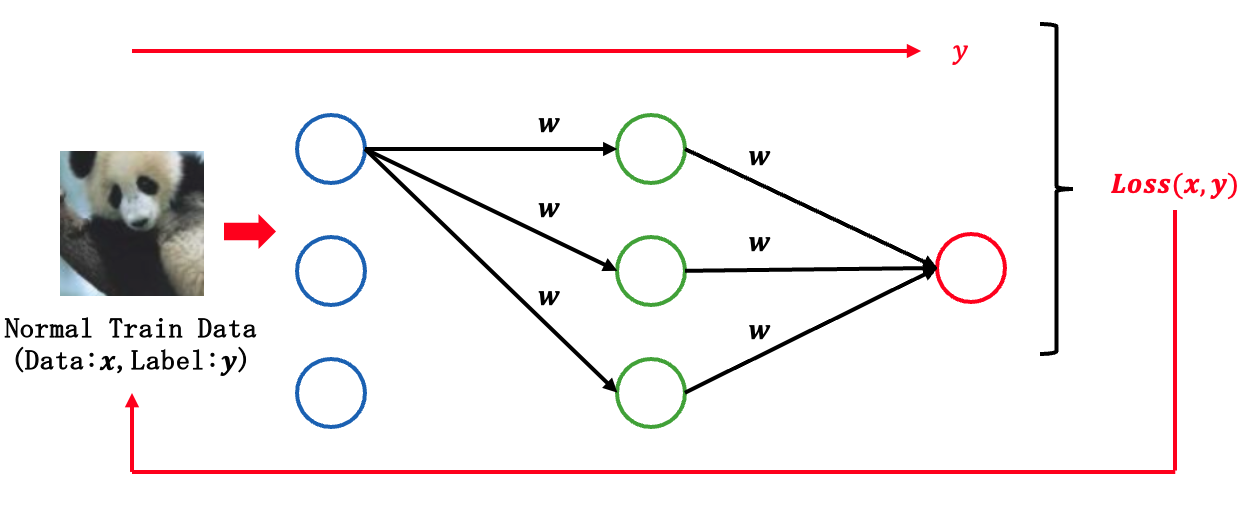
\includegraphics[width=0.8\textwidth]{images/敵対的学習1.png}
        \caption{敵対的学習1:敵対的サンプルを生成}
        \label{fig:adversarial_learning1}
    \end{figure}
    
    \item 機械モデルに正常なデータ $\bm{x}$ と敵対的サンプル $\bm{x}'$ を入力し,それぞれの誤差 $Loss$ を得る

    図2は,生成された敵対的サンプルと元データとの入力の違いを比較している.元データは,すべて純粋な特徴量から構成され,モデルが意図通りに分類などを行うための基盤となる.一方敵対的サンプルは,元データに対して微細なノイズを加えたもので,このノイズはほとんど人間には認識できないものである.しかしモデルの分類結果を大きく変えてしまうため入力の誤差を出力している.

    \begin{figure}[H]
        \centering
        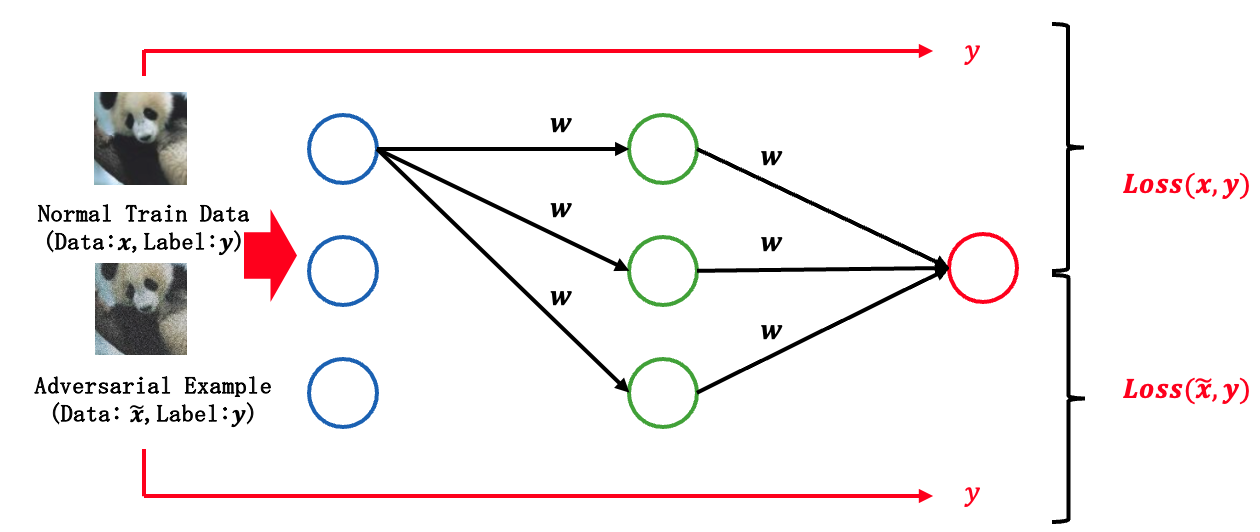
\includegraphics[width=0.8\textwidth]{images/敵対的学習2.png}
        \caption{敵対的学習2:元データと敵対敵サンプルの誤差の導出}
        \label{fig:adversarial_learning2}
    \end{figure}

    \item それぞれ得た誤差 $Loss(x, y), Loss(x', y)$ に重み係数 $\alpha$ をつけて足し合わせる

    図3では,元データによって生成された誤差と敵対的サンプルによって生成された誤差を取得し,足し合わせている.この誤差をどのようなバランスで機械学習モデルに組み込んでいくかという重要なステップである. 上記の式(1)にある誤差の足し合わせの式用いて行われる。
    
    \begin{figure}[H]
        \centering
        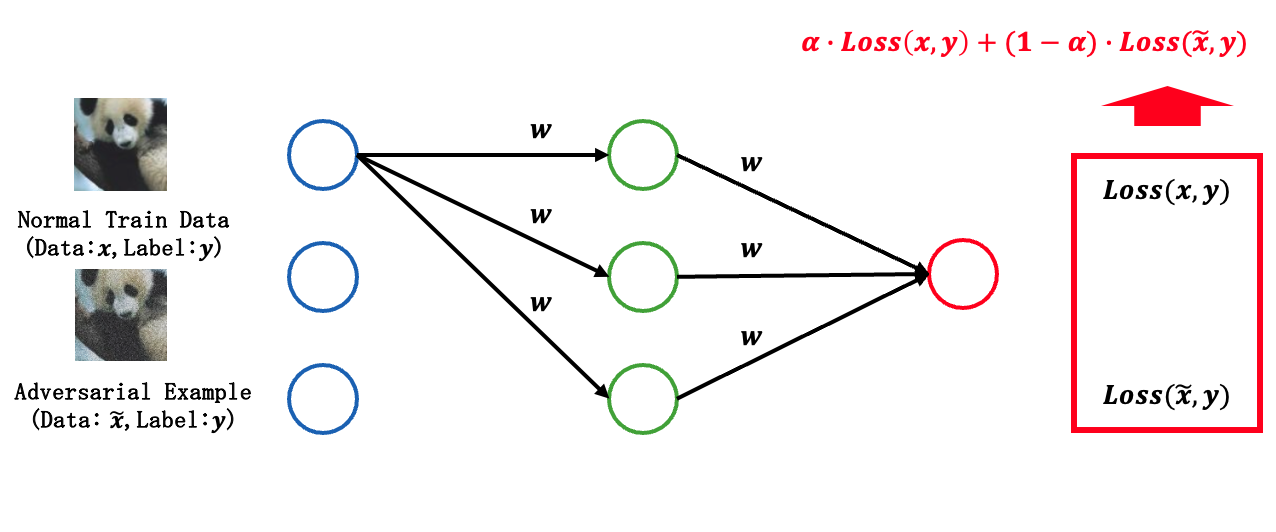
\includegraphics[width=0.8\textwidth]{images/敵対的学習3.png}
        \caption{敵対的学習3:元データと敵対敵サンプルの誤差の足し合わせ}
        \label{fig:adversarial_learning3}
    \end{figure}

    \item 足し合わされた誤差 $Loss$ が最小となるように,重み $\bm{w}$ を更新する

    図4では,先ほど生成された敵対的サンプルの誤差を含めた誤差を用いて,機械学習モデルの更新を行う.この作業は敵対的サンプルによる誤分類にも耐えられるような分類を行うために図1で学習された機械学習モデルの重み $w$ を敵対的サンプルに対応させるため更新する.
    先ほどの式(1)を最小化することで,重み $w$ を $w_{\_new}$ に更新する.これにより,敵対的サンプルの挙動を抑えることができた機械学習モデルを作成することができる.
    
    \begin{figure}[H]
        \centering
        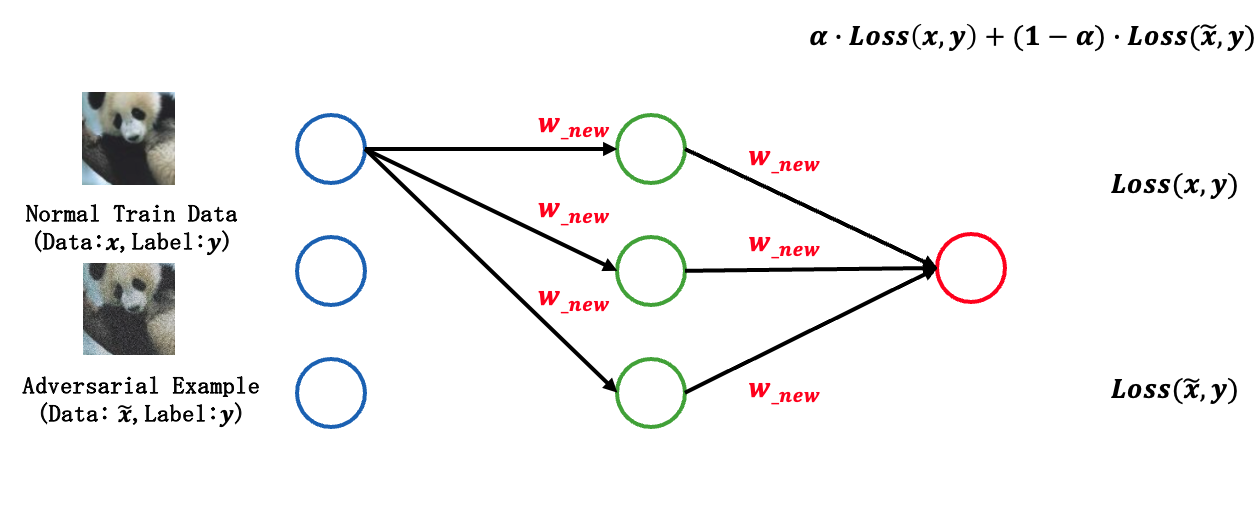
\includegraphics[width=0.8\textwidth]{images/敵対的学習4.png}
        \caption{敵対的学習4:重みの更新}
        \label{fig:adversarial_learning4}
    \end{figure}

\end{enumerate}

以上の流れにより,敵対的サンプルを学習過程の中に組み込むような敵対的学習を行うことで,機械学習モデルが敵対的サンプルの挙動に対応することができ,堅牢性を向上させることができる.

\subsection{敵対的サンプル}
敵対的学習を実現する上で中心となるのが,敵対的サンプルの生成である.ここでは,敵対的サンプルがどのようにモデルに影響を与えるかを詳しく説明する.
研究背景で触れたように敵対的サンプルとは,人間には見分けのつかない微細なノイズをデータに付与することで機械学習モデルの誤分類を引き起こすデータである.\cite{MBSD-AdversarialExample}運用している機械学習モデルを狙った攻撃に使用されることがある.

敵対的サンプルによる誤分類を確認した実験をGoodfellowらが行っている\cite{goodfellow2015explaining}.
\begin{figure}[H]
    \centering
    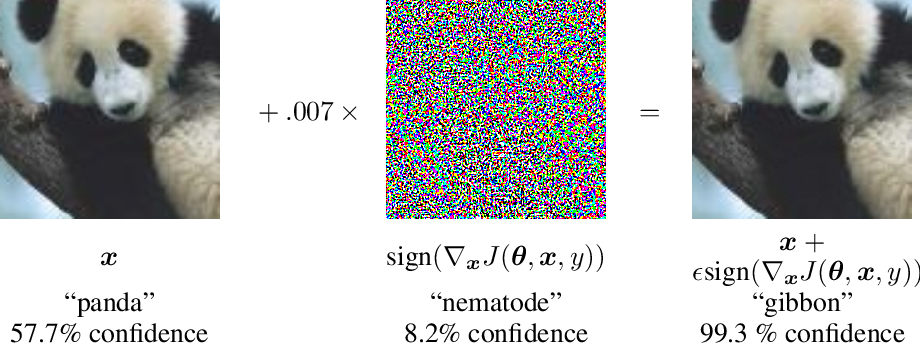
\includegraphics[width=0.8\textwidth]{images/goodfellow_panda.png}
    \caption{敵対的サンプルの例:パンダの敵対的サンプル画像をテナガザルと判断\cite{goodfellow2015explaining}}
    \label{fig:adversarial_example}
\end{figure}

図5は,敵対的サンプルの具体例として,パンダの画像に微細なノイズを加えた結果,モデルがテナガザルと誤分類した事例を示している.この例は,敵対的サンプルが人間にはほとんど判別できない変更であっても,モデルにとっては大きな影響を与えることを視覚的に示しています.

このように画像データに対する敵対的サンプルの生成は行うことができることがわかった.しかし,表形式データに対する敵対的サンプルは,先ほどの手法を用いて生成することは難しいという問題がある.その理由として,表形式データの特徴量は画像データと異なる性質を持つためである.画像データの場合,各ピクセルの値は0から255の範囲の連続値として扱うことができ,わずかな変化は人間の目では認識できないことが多い.一方で,表形式データの特徴量には,年齢や収入といった数値データだけでなく,性別や職業といったカテゴリカル変数も含まれる.また,各特徴量は独立した意味を持っており,それぞれの特徴量の変化は明確な意味の変化を伴う.例えば,先ほどのパンダの画像の場合,個々のピクセル値にわずかな変化を加えても,人間にとってはそれが「パンダの画像」であることに変わりはない.しかし,ローン申請データにおいて,年収を示す特徴量に対してわずかな変化を加えた場合,その変化は申請者の経済状況を直接的に変えてしまう可能性がある.さらに,職業などのカテゴリカルデータの場合,わずかな変化という概念自体が適用できない.このような表形式データの特性により,画像データに対する敵対的サンプル生成手法をそのまま適用することは適切ではない.そこで,表形式データの特性を考慮した新たな敵対的サンプル生成手法が必要となる.特に,各特徴量の重要度や,特徴量の種類(連続値かカテゴリカル値か)を考慮した手法が求められる.


